\section{Frequentist Statistics}
\label{chp:freq}
Frequentist statistics is based on \dfref{def:frequentist_statistics}, which follows the definition of objective probability (\dfref{def:objective_probability}) and the principle of fixed, unknown parameters (\axref{ax:parameter_fixed}). The foundations of Frequentist statistics trace back to seminal works such as those of Neyman and Pearson \citep{Neyman1928OnSR} and Fisher \citep{fisher1925statistical}, who laid the groundwork for much of its methodology. Subsequent developments by Wald \citep{Wald1945Sequential}, Neyman \citep{Neyman1948Consistent}, and Lehmann \citep{lehmann1986testing} further refined its theories and techniques.\newline

In the Frequentist paradigm, it is assumed that Nature's actions are generated by a model with parameters $w \in \Omega_W$, which are unknown but fixed. In this setting, the optimal decision rule can be expressed as
\begin{equation}
	U^*(x,w).
\end{equation}
Thus, all quantities in \secref{sec:framing_statistics} become conditioned on $w$. Since $w$ is not known to the Robot, the central task becomes to estimate $w$ from past data $D$. 

This gives rise to a nested decision problem with two levels:
\begin{enumerate}
	\item[\textit{i)}] Parameter estimation: use past data $D$ to construct an estimator $\hat{w}(D)$ of the fixed but unknown parameter $w$.
	\item[\textit{ii)}] Prediction/decision: given a new observation $x$ and the parameter estimate $\hat{w}(D)$, apply the decision rule $U$ to determine an action.
\end{enumerate}

To avoid notational ambiguity, a distinction is made between the decision rule used for prediction, denoted $U$, and the decision rule used for parameter estimation, denoted $\hat{w}$. The practical decision rule for a new observation $x \in \Omega_X$ therefore takes the form
\begin{equation}
	U^*(x, \hat{w}^*(D)),
\end{equation}
where $\hat{w}^*(D)$ denotes the optimal parameter decision rule, obtained from past data $D$, and the final action is determined by minimizing the expected cost as specified in \secref{sec:framing_statistics}.



\subsection{Frequentist Regression}
\label{chp:frequentist_regression}
In the Frequentist paradigm, regression involves the Robot constructing a model $f: \Omega_W \times \Omega_X \mapsto \mathbb{R}$, parameterized by $w \in \Omega_W$, to approximate Nature's actions $s\in \Omega_S$ based on observed data $x\in \Omega_X$. As in Bayesian regression (\secref{chp:regression}), the output of $f$ is real-valued, so that $S$ is assumed continuous. The model $f$ serves as the Robot's surrogate for Nature's mechanism, providing predictions of Nature's action given observed data $x \in \Omega_X$. \newline

Suppose Nature's action $s\in\Omega_S$ given observed data $x\in \Omega_X$ is distributed according to a normal distribution with mean $f(w,x)$ and precision $\xi \in \Omega_{\Xi}$,
\begin{equation}
	p(s | x, w, \xi, I) 
	= \sqrt{\frac{\xi}{2\pi}} e^{-\frac{\xi}{2}(f(w,x)-s)^2}.
	\label{freq:dist}
\end{equation}
Here, $(w,\xi)$ are fixed but unknown parameters. Under the quadratic cost function from \dfref{def:quadratic_cost}, the optimal decision rule is the conditional expectation of $S$ given $(x,w,\xi)$ (\thref{theorem:expectation_decision_rule}),
\begin{equation}
	\begin{split}
		U^*(x,\hat{w}^*(D),\hat{\xi}^*(D)) &= \mathbb{E}[S | x, \hat{w}^*(D), \hat{\xi}^*(D), I]\\
		&= \int s p(s | x, \hat{w}^*(D), \hat{\xi}^*(D), I) ds\\
		& = f(\hat{w}^*(D),x).
	\end{split}
	\label{freq:decision}
\end{equation}
\EQref{freq:decision} represents the Frequentist optimal decision rule conditional on the parameter estimate, whereas \EQref{eq:q3} represents the Bayesian optimal decision rule, which averages over the posterior distribution of the model parameters (and latent variables) given the data. From equation \EQref{freq:decision} it is clear that in Frequentist statistics, regression is reframed as parameter estimation.


\subsection{Frequentist Classification}
\label{chp:frequentist_classification}

In the Frequentist paradigm, classification involves the Robot constructing a model
\begin{equation}
	f: \Omega_W \times \Omega_X \mapsto \Delta^K, \quad w \in \Omega_W,
\end{equation}
where $\Delta^K$ is the $K$-dimensional probability simplex and $\Omega_S \in \{1,\dots,K\}$ represents Nature's discrete action (class label). The model predicts the conditional probability of each class given the input $x \in \Omega_X$:
\begin{equation}
	p(S = s | x, w, I) = f_s(w, x), \quad s \in \{1,\dots,K\},
\end{equation}
with
\begin{equation}
	\sum_{s\in \Omega_S} p(S = s | x, w, I) = 1.
\end{equation}
The Robot's action space is typically equal to Nature's action space, $\Omega_U = \Omega_S$, possibly with the addition of a reject option at cost $\lambda$. Using the 0--1 cost function with optional reject,
\begin{equation}
	C(U(x,w), s) = 1 - \delta_{U(x,w),s} + (\lambda-1)\delta_{U(x,w), \text{"Reject"}}.
\end{equation}
Let $\hat{w}^*(D)$ denote the optimal Frequentist estimator of the model parameters obtained from past data $D$. The optimal decision rule for a new observation $x$ is
\begin{equation}
	\begin{split}
		U^*(x, \hat{w}^*(D)) &= \arg\min_{u \in \Omega_U} \mathbb{E}[C(u, S) \mid x, \hat{w}(D), I] \\
		&= \arg\min_{u \in \Omega_U} \Big(1 - f_{u}(\hat{w}^*(D), x) + (\lambda-1)\delta_{u, \text{"Reject"}}\Big).
	\end{split}
	\label{freq:decision_classification}
\end{equation}
From equation \EQref{freq:decision_classification} it is clear that in Frequentist statistics, classification is reframed as parameter estimation.


\subsection{Frequentist Parameter Estimation}
\label{chp:frequentist_parameter_estimation}
As shown in \secref{chp:frequentist_regression} and \secref{chp:frequentist_classification}, both regression and classification in the Frequentist paradigm can be reframed as problems of parameter estimation. This makes parameter estimation the central focus of Frequentist statistics. Unlike in Bayesian statistics, where parameters are intermediate quantities to be marginalized over, in the Frequentist framework the parameters are fixed but unknown, and their determination carries substantive interpretational and practical importance. Estimators of these parameters serve as decision rules that summarize past observations into actionable predictions.

\begin{definition}[Fisher Information]
	\label{def:fisher_information}
	Take $D_s= \{s_i\}_{i=1}^n$, $D_x= \{x_i\}_{i=1}^n$ and let $w \in \Omega_W$ be an unknown parameter of the model. Let $p(D_s | D_x, w, I)$ denote the likelihood of observing Natures actions $D_s$ given observed data $D_x$ and $w$. The Fisher information is defined as
	\begin{equation}
		\begin{split}
			\mathcal{I}(w) &\equiv \mathbb{E} \bigg[\bigg(\frac{\partial}{\partial w} \ln p(D_s|D_x, w,I)\bigg)^2 \Bigg| D_x, w,I\bigg]\\
			&= \operatorname{Var}\bigg[\frac{\partial}{\partial w} \ln p(D_s|D_x, w,I) \Bigg| D_x, w,I\bigg].
		\end{split}
	\end{equation}
\end{definition}

\begin{proof}
	In general
	\begin{equation}
		\mathbb{E}\bigg[\bigg(\frac{\partial}{\partial w} \ln p\bigg)^2\bigg] 
		= \operatorname{Var}\bigg[\frac{\partial}{\partial w} \ln p\bigg] + 
		\bigg(\mathbb{E}\bigg[\frac{\partial}{\partial w} \ln p\bigg]\bigg)^2.
	\end{equation}
	Now
	\begin{align}
		\mathbb{E}\bigg[\frac{\partial}{\partial w} \ln p\bigg] 
		&= \int dD_s  \bigg(\frac{\partial}{\partial w} \ln p\bigg)  p \\
		&= \int dD_s  \frac{\partial}{\partial w} p \\
		&= \frac{\partial}{\partial w} \int dD_s  p \\
		&= 0,
	\end{align}
	since $\int dD_s \, p(D_s \mid D_x, w, I) = 1$. Therefore
	\begin{equation}
		\mathcal{I}(w) = \operatorname{Var}\bigg[\frac{\partial}{\partial w} \ln p(D_s \mid D_x, w, I) \bigg| D_x, w, I\bigg].
	\end{equation}
\end{proof}

\begin{theorem}[Fisher Information for Independent Observations]
	\label{thm:fisher_sample}
	Take $D_s= \{s_i\}_{i=1}^n$ , $D_x = \{x_i\}_{i=1}^n$ and let $w \in \Omega_W$ be a parameter of the model. Assume the likelihood factorizes as
	\begin{equation}
		p(D_s | D_x, w, I) = \prod_{i=1}^{n} p(s_i | x_i, w, I).
	\end{equation}
	Then, the Fisher information of the full dataset is
	\begin{equation}
		\mathcal{I}(w) 
		= \mathbb{E}\Bigg[\Big(\frac{\partial}{\partial w} \ln p(D_s | D_x, w, I)\Big)^2 \Bigg| D_x, w, I \Bigg] 
		= \sum_{i=1}^{n} \mathcal{I}_i(w),
	\end{equation}
	where $\mathcal{I}_i(w)$ is the Fisher information of the $i$-th observation:
	\begin{equation}
		\mathcal{I}_i(w) = \mathbb{E}\Bigg[\Bigg(\frac{\partial}{\partial w} \ln p(s_i | x_i, w, I)\Bigg)^2 \Bigg| x_i, w, I \Bigg].
	\end{equation}
\end{theorem}


\begin{definition}[Maximum Likelihood Estimator (MLE) Decision Rule]
	\label{def:MLE}
	Take $D_s= \{s_i\}_{i=1}^n$ , $D_x = \{x_i\}_{i=1}^n$ and let $w \in \Omega_W$ be a fixed but unknown parameter. The Maximum Likelihood Estimator (MLE) decision rule $\hat{w}_{\mathrm{MLE}}$ is the value of $w$ that maximizes the likelihood of observing $D_s$ given $D_x$
	\begin{equation}
		\hat{w}_{\mathrm{MLE}}(D) \equiv \arg \max_{w \in \Omega_W} p(D_s | D_x, w, I),
	\end{equation}
	where $I$ denotes the background information.
\end{definition}


\begin{theorem}[Asymptotic Unbiasedness of the MLE]
	\label{thm:unbiased_mle}
	Under standard regularity conditions, the MLE $\hat{w}_{\mathrm{MLE}}$ is asymptotically unbiased and normally distributed:
	\begin{equation}
		\sqrt{n}\,\big(\hat{w}_{\mathrm{MLE}} - w\big) \xrightarrow{\text{d}} \mathcal{N}\big(0, \mathcal{I}(w)^{-1}\big),
	\end{equation}
	where $\mathcal{I}(w)$ is the Fisher information matrix evaluated at $w$ and $\xrightarrow{\text{d}}$ denotes convergence in distribution as $n \to \infty$.
\end{theorem}

\begin{definition}[Minimax Decision Rule]
	\label{def:minimax}
	A decision rule $\hat{w}'$ is said to be minimax if it minimize the maximum expected cost, meaning (\EQref{eq:conditional_expected_cost})
	\begin{equation}
		\begin{split}
			\hat{w}' &\equiv \inf_{\hat{w}}\sup_{w\in \Omega_W}\mathbb{E}[C(\hat{w},w)|w,I]\\
			& = \inf_{\hat{w}}\sup_{w\in \Omega_W}\int dD  C(\hat{w}(D),w) p(D|w,I).
		\end{split}
	\end{equation}
\end{definition}


\begin{theorem}[Mean Squared Error (MSE)]
	\label{theorem:MSE}
	The expectation of the quadratic cost function (\dfref{def:quadratic_cost}) can be written
	\begin{equation}
		\begin{split}
			\mathbb{E}[C(\hat{w}, w)|w,I] &= \mathbb{E}[(\hat{w}-w)^2|w,I]\\ 
			&= \mathbb{E}[(\hat{w}-\mathbb{E}[\hat{w}|I])^2|w,I]+(w-\mathbb{E}[\hat{w}|I])^2\\
			&=\operatorname{Var}[\hat{w}|w,I]+\operatorname{Bias}[\hat{w}|w,I]^2\\
		\end{split}
		\label{eq:MSE}
	\end{equation}
	where conditions have been suppressed in the second line (to fit to the page) and the bias of the estimator of $\hat{w}$ is defined viz
	\begin{equation}
		\text{Bias}[\hat{w}|w,I]\equiv w-\mathbb{E}[\hat{w}|I].
	\end{equation}
	If $\mathbb{E}[C(\hat{w}, w)|w,I] \to 0$ as $n \to \infty$, then $\hat{w}$ is a weakly consistent estimator of $w$, i.e., $\hat{w} \xrightarrow{p} w$. There can be different consistent estimates that converge towards $w$ at different speeds. It is desirable for an estimate to be consistent and with small (quadratic) cost, meaning that both the bias and variance of the estimator should be small. In many cases, however, there is bias-variance which means that both cannot be minimized at the same time. 
\end{theorem}

\begin{corollary}[MLE is Approximately Minimax for quadratic Loss]
	\label{cor:MLE_minimax}
	Under certain regularity conditions, the Maximum Likelihood decision rule (MLE) $\hat{w}_{\text{MLE}}$ is approximately minimax for the quadratic cost function (\dfref{def:quadratic_cost}), meaning it approximately minimizes the maximum expected cost.
	
	\begin{proof}
		From theorem \thref{theorem:MSE}
		\begin{equation}
			\mathbb{E}[(\hat{w}-w)^2|w,I] = \operatorname{Var}[\hat{w}|w,I]+\operatorname{Bias}[\hat{w}|w,I]^2.
		\end{equation}
		Under the regularity conditions where the MLE is unbiased and has asymptotically minimal variance, the bias term vanish, meaning $\operatorname{Bias}[\hat{w}_{\text{MLE}}|w,I] = 0$ and the variance term $\operatorname{Var}[\hat{w}_{\text{MLE}}|w,I]$ is minimized among a class of estimators. Thus, the expected quadratic cost for the MLE can be approximated by
		\begin{equation}
			\begin{split}
				\mathbb{E}[(\hat{w}_{\text{MLE}}-w)^2|w,I] &\approx \operatorname{Var}[\hat{w}_{\text{MLE}}|w,I]\\
				&\approx \frac{\operatorname{tr}[\mathcal{I}(w)^{-1}]}{n},
			\end{split}
		\end{equation}
		where \thref{thm:unbiased_mle} was used for the second line. The Cramer-Rao lower bound~\citep{Rao1973Linear} for variance states that 
		\begin{equation}
			\operatorname{Var}[\hat{w}|w,I]\geq \frac{\text{tr}[\mathcal{I}(w)^{-1}]}{n},
		\end{equation}
		implying that the MLE decision rule acheives the smallest possible variance asymptotically and therefore that 
		\begin{equation}
			\sup_{w\in \Omega_W}\mathbb{E}[(\hat{w}_{\text{MLE}}-w)^2|w,I]\approx \inf_{\hat{w}} \sup_{w \in \Omega_W} \mathbb{E}[(\hat{w} - w)^2|w,I],
		\end{equation}
		meaning the MLE decision rule is approximately the minimax decision rule under quadractic cost.
	\end{proof}
\end{corollary}

\begin{example}
	The bias-variance decomposition (\thref{theorem:MSE}) is a concept relevant to Frequentist statistics, where a single point estimate of the parameters is used. This decomposition illustrates the tradeoff between underfitting and overfitting: high bias corresponds to underfitting, while high variance corresponds to overfitting. \newline
	
	In Bayesian statistics, predictions are obtained by integrating over the posterior distribution of parameters, rather than relying on a single point estimate. This integration inherently regularizes the model, mitigating overfitting and underfitting.
\end{example}


\begin{example}
	Take $D_s= \{S = s_i\}_{i=1}^n$ with $S \sim \mathrm{Ber}(w)$, and let $w\in [0,1]$ be the unknown parameter. Determine the quadratic cost of three different decision rules for estimating $w$: the arithmetic sample mean, the constant $0.5$, and the first observation $s_1$.
	
	\begin{itemize}
		\item Arithmetic mean:
		\begin{equation}
			\hat{w}(D_s) = \frac{1}{n} \sum_{i=1}^n s_i
		\end{equation}
		with
		\begin{equation}
			\begin{split}
				\mathbb{E}[\hat{w}(D_s)|w,I] &= \frac{1}{n} \sum_{i=1}^n \mathbb{E}[S|w,I] = w,\\
				\operatorname{Var}[\hat{w}(D_s)|w,I] &= \frac{1}{n^2} \sum_{i=1}^n \operatorname{Var}[S|w,I] = \frac{w(1-w)}{n},\\
				\mathbb{E}[(\hat{w}(D_s)-w)^2|w,I] &= \operatorname{Var}[\hat{w}(D_s)|w,I] = \frac{w(1-w)}{n}.
			\end{split}
		\end{equation}
		
		\item Constant estimate:
		\begin{equation}
			\hat{w} = 0.5
		\end{equation}
		with
		\begin{equation}
			\begin{split}
				\mathbb{E}[\hat{w}|w,I] &= 0.5,\\
				\operatorname{Var}[\hat{w}|w,I] &= 0,\\
				\mathbb{E}[(\hat{w}-w)^2|w,I] &= (0.5 - w)^2.
			\end{split}
		\end{equation}
		
		\item First observation:
		\begin{equation}
			\hat{w}(D_s) = s_1
		\end{equation}
		with
		\begin{equation}
			\begin{split}
				\mathbb{E}[\hat{w}(D_s)|w,I] &= \mathbb{E}[S|w,I] = w,\\
				\operatorname{Var}[\hat{w}(D_s)|w,I] &= \operatorname{Var}[S|w,I] = w(1-w),\\
				\mathbb{E}[(\hat{w}(D_s)-w)^2|w,I] &= w(1-w).
			\end{split}
		\end{equation}
	\end{itemize}
	
	The arithmetic mean minimizes the quadratic cost over the entire range of $w$, while the constant $0.5$ performs better for specific values of $w$. The cost of using $s_1$ is independent of $n$, making it less favorable as the sample size increases.
	
	\begin{figure}[H]
		\captionsetup{width=1\textwidth}
		\centering
		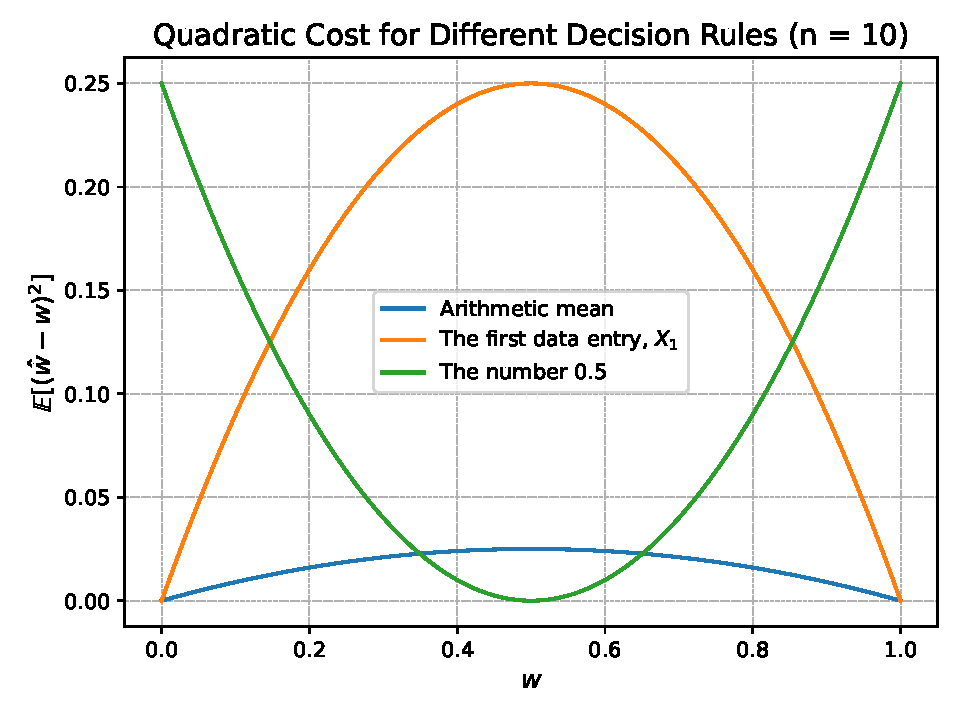
\includegraphics[width=1\textwidth]{figures/ber_example.pdf}
		\caption{Quadratic cost, $\mathbb{E}[(\hat{w} - w)^2|w,I]$, for three decision rules: arithmetic mean (blue), first observation $s_1$ (orange), and constant $0.5$ (green).}
		\label{fig:pen}
	\end{figure}
\end{example}


\begin{example}
	Take $D_s= \{S= s_i\}_{i=1}^n$ with $S\sim \mathrm{Ber}(w)$, and let $w\in [0,1]$ be the unknown parameter. Determine the maximum likelihood estimate of $w$.\newline
	
	\noindent In this case
	\begin{equation}
		\begin{split}
			p(D_s|D_x,w,I) & =p(D_s|w,I)\\
			& = \prod_{i=1}^nw^{s_i}(1-w)^{1-s_i}.
		\end{split}
	\end{equation}
	Let $l(w)\equiv \ln p(D_s|D_x,w,I)$, then
	\begin{equation}
		\begin{split}
			\argmax_wl(w) & = \argmax_wp(D_s|w,I)\\
			&= \argmax_w\ln \bigg(\prod_{i=1}^nw^{s_i}(1-w)^{1-s_i}\bigg)\\
			&=\argmax_w \bigg[\ln w\sum_{i=1}^ns_i + \ln(1-w)\sum_{i=1}^n(1-s_i)\bigg]
		\end{split}
	\end{equation}
	Now 
	\begin{equation}
		\frac{d}{dw}l(w)=\frac{\sum_{i=1}^ns_i}{w}-\frac{n-\sum_{i=1}^ns_i}{1-w}
	\end{equation}
	Requiring the derivative to vanish means the maximum likelihood estimate of $w$ is given by
	\begin{equation}
		\hat{w}_{\text{MLE}}(D_s)=\frac{1}{n}\sum_{i=1}^ns_i.
	\end{equation}
\end{example}
\begin{example}
	Take $D_s= \{S = s_i\}_{i=1}^n$ with $S\sim \mathrm{Exp}(w)$, and let $w> 0$ be the unknown parameter. Determine the maximum likelihood estimate of $w$.\newline
	
	\noindent In this case
	\begin{equation}
		\begin{split}
			p(D_s|D_x,w,I)& =p(D_s|w,I)\\
			& =\prod_{i=1}^nw e^{-w s_i}.
		\end{split}
	\end{equation}
	Let $l(w)\equiv \ln p(D_s|D_x,w,I)$, then
	\begin{equation}
		\frac{d}{dw}l(w)=\frac{n}{w}-\sum_{i=1}^ns_i
	\end{equation}
	Requiring the derivative to vanish means the maximum likelihood estimate of $w$ is given by
	\begin{equation}
		\hat{w}_{\text{MLE}}(D_s)=\frac{1}{\frac{1}{n}\sum_{i=1}^ns_i}.
	\end{equation}
\end{example}

